%laden der Präambel mit Latexbefehlen/-klassen
% !TeX encoding = UTF-8

\documentclass[a0paper,landscape]{baposter}
\usepackage[english]{babel}
\usepackage[utf8]{inputenc}
%\usepackage{arev}
%\usepackage[T1]{fontenc}

\usepackage{marvosym}
\usepackage{pifont}
\usepackage{setspace}

\usepackage{makecell}

%for mathematical symbols
\usepackage{amsmath}
\usepackage{amsxtra}
\usepackage{eurosym}
\usepackage{siunitx}  
\sisetup{locale=DE}
\usepackage[version=4]{mhchem}

%Typography
\usepackage[auto]{microtype}

\usepackage{booktabs}
\usepackage{multirow}
\usepackage{paralist}

\usepackage[
backend=biber,
style=nature,
citestyle=numeric-comp,
sorting=none,
maxbibnames=1,
firstinits=true
]{biblatex}
%\usepackage{natbib}

\bibliography{biblio/refs,biblio/bibtemp}
\setlength\bibitemsep{2.5pt}

%colors
\definecolor{standardfontcolor}{RGB}{0,0,0} 
\definecolor{bordercol}{RGB}{113,113,113}
\definecolor{headercol1}{RGB}{255,255,255}
\definecolor{headercol2}{RGB}{113,113,113}
\definecolor{headerfontcol}{RGB}{0,0,0}
\definecolor{boxcolor}{RGB}{255,255,255}


\begin{document}
	\typeout{Poster rendering started}
	
\background{
	\begin{tikzpicture}[remember picture,overlay]%
	\draw (current page.north west)+(-2em,2em) node[anchor=north west]
	{\includegraphics[height=1.1\textheight]{figures/background}};
	\end{tikzpicture}
}

\color{standardfontcolor}

\begin{poster}{
		grid=false,
		columns=3,
		%colspacing=length
		headerheight=0.125\textheight,
		eyecatcher=false,
        borderColor=bordercol,
		headerColorOne=headercol1,
		headerColorTwo=headercol2,
		headerFontColor=headerfontcol,
		% Only simple background color used, no shading, so boxColorTwo isn't necessary
		boxColorOne=boxcolor,
		headershape=roundedright,
		headerfont=\sffamily\bfseries\Large,
		textborder=rectangle,
		headerborder=open,
		boxshade=plain,
		background=none
%		background=user
	}
	%%% Eye Cacther %%%%%%%%%%%%%%%%%%%%%%%%%%%%%%%%%%%%%%%%%%%%%%%%%%%%%%%%%%%%%%%
	{
		Eye Catcher, empty if option eyecatcher=false - unused
	}
%----------------------------------------------------------------------------------------
%	TITLE AND AUTHOR NAME
%----------------------------------------------------------------------------------------
%
{
	\textsf %Sans Serif
	{\vskip 2.0cm \huge Exploraci\'on de escenarios f\'isicos de ruptura s\'ismica \\ en sistemas complejos de fallas normales
	}
}
{\sf\vspace{-0.1em}\\
	{\textbf{H.-S. S\'anchez-Reyes$^1$}, O. Scotti$^2$, S. Hok$^2$, A.-A. Gabriel$^3$ and T. Taufiqurrahman$^3$}
	\vspace{0.6em}\\
	\normalsize{$^1$Institut des Sciences de la Terre, IRD-UGA, BP 53, 38041 Grenoble Cedex 9, France \vspace{0.1em}\\
	$^2$Bureau d’Évaluation des Risques Sismiques pour la Sûreté des Installations, IRSN, 92260 Fontenay-aux-Roses, France
	\vspace{0.1em}\\
	$^3$Department of Earth and Environmental Sciences, Ludwig-Maximilians-Universitat, 80333 Munchen, Germany	 	
	} \\ \\ \\ \\ \\ 
}
% University/lab logo
{ \begin{minipage}{2cm}
  \vskip -0.2cm \hskip -5.2cm 
\includegraphics[width=7.1cm]{../../../logos/logo_poster_2022.png} \\
 \end{minipage}
 }

 

\headerbox{{\bf 1.} Introducci\'on}{name=intro,column=0,row=0,span=1}{

\begin{minipage}{0.4\linewidth}
 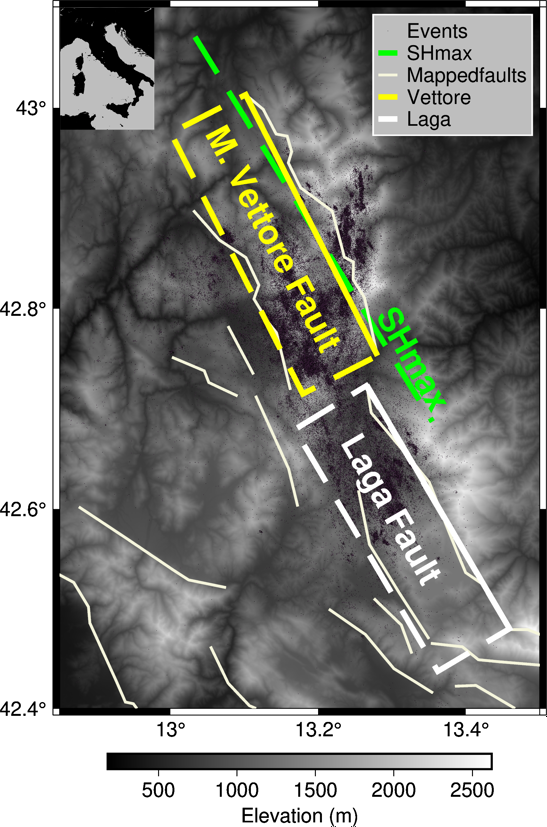
\includegraphics[width=1\linewidth]{images/Map_Italy}
\end{minipage}
\begin{minipage}{0.58\linewidth}
 \vskip -0.2cm {{\bf Contexto geol\'ogico:}} \\
 \vskip -0.2cm
 {\small Italia Central (Apeninos):}
 {\small
 \begin{itemize}
  \item Sistema de fallas Normales
  \item Rupturas a lo largo de \\
        m\'ultiples segmentos \\
 \end{itemize}
 } \vskip -0.2cm
 {\small Riesgo s\'ismico):}
 {\small
 \begin{itemize}
  \item Ciudades cercanas
  \item Terremotos Mw$>$5
  \item Profundidad $<$12 km
 \end{itemize}
 } 
\end{minipage} \\
 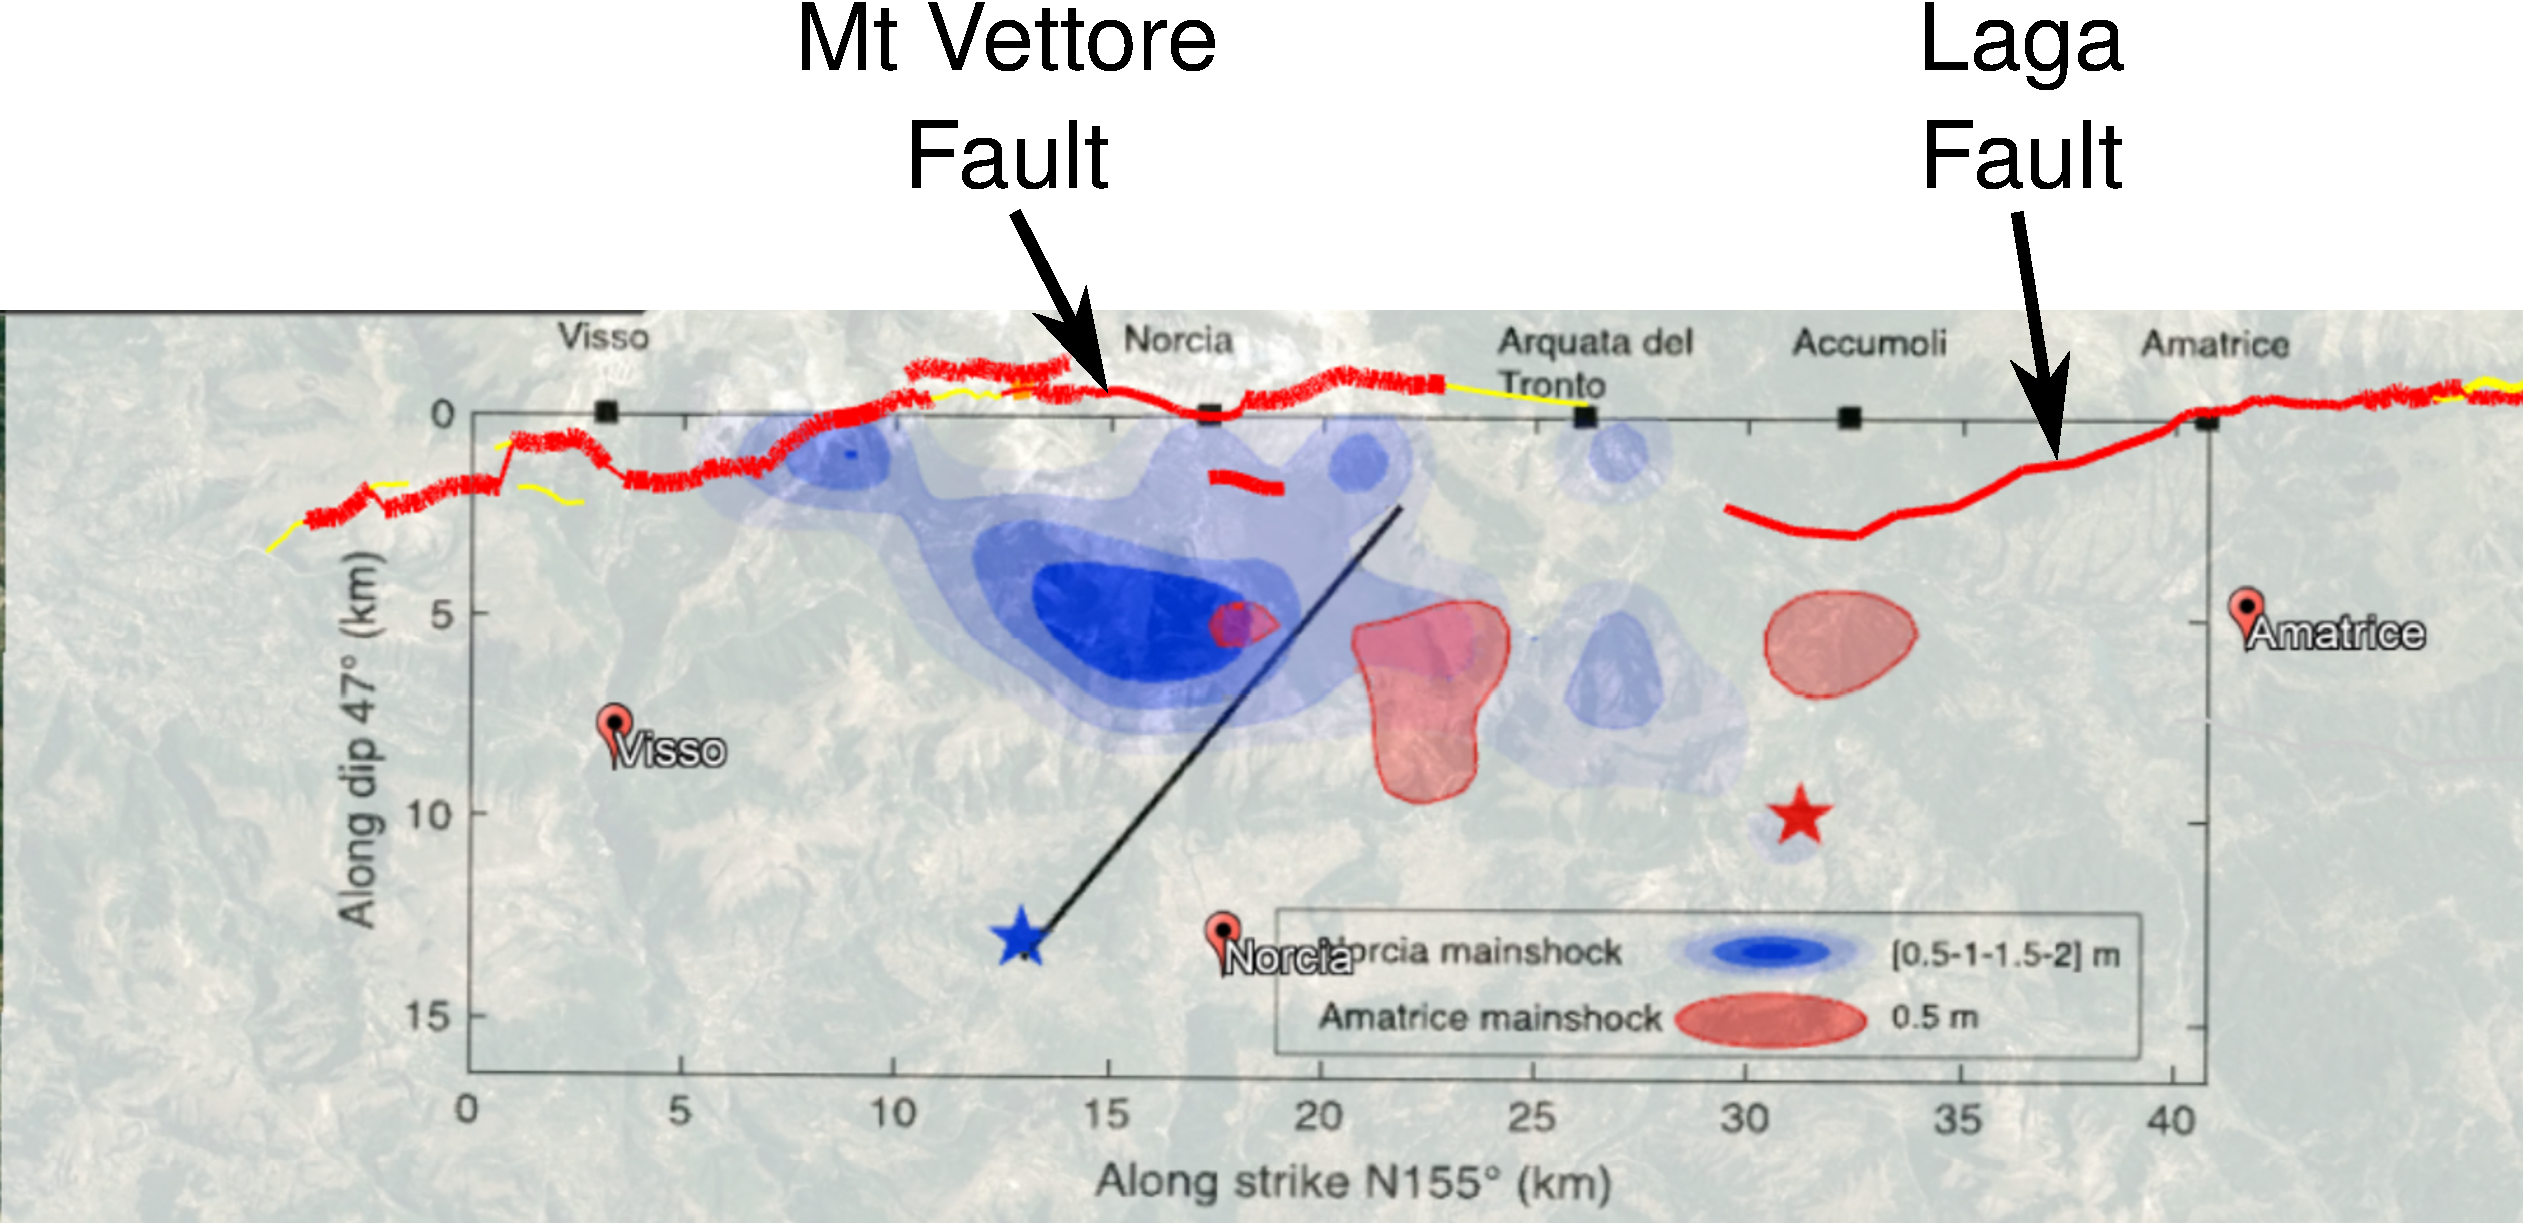
\includegraphics[width=1\linewidth]{images/amatrice_1-crop.pdf}


\vskip 0.2cm
   \begin{tikzpicture}[%
    auto,
    block/.style={
      rectangle,
      draw=red!200,
      thick,
      fill=none,
      text width=0.95\textwidth,
      align=justify,
      rounded corners,
      minimum height=4em,
      minimum width=1\linewidth
    },
    block1/.style={
      rectangle,
      draw=black,
      thick,
      fill=red!20,
      text width=\textwidth,
      align=center,
      rounded corners,
      minimum height=4em
    },
    line/.style={
      draw,thick,
      -latex',
      shorten >=4pt
    },
    cloud/.style={
      draw=red,
      thick,
      elipse,
      fill=red!20,
      minimum height=4em
    }
  ]
    \draw (2.5,-2) node[block] (C) {
    \bf \color{red} \small Objetivo: Investigar qu\'e par\'ametros f\'isicos promueven
    el salto de una ruptura s\'ismica. Mejorar la estimaci\'on
    del riesgo s\'ismico asociado.};     


  \end{tikzpicture} \vskip -0.2cm



}


\headerbox{{\bf 2.} Geometr\'ia y par\'ametros}{name=geo,column=0,row=1,span=1,below=intro}{

\centering 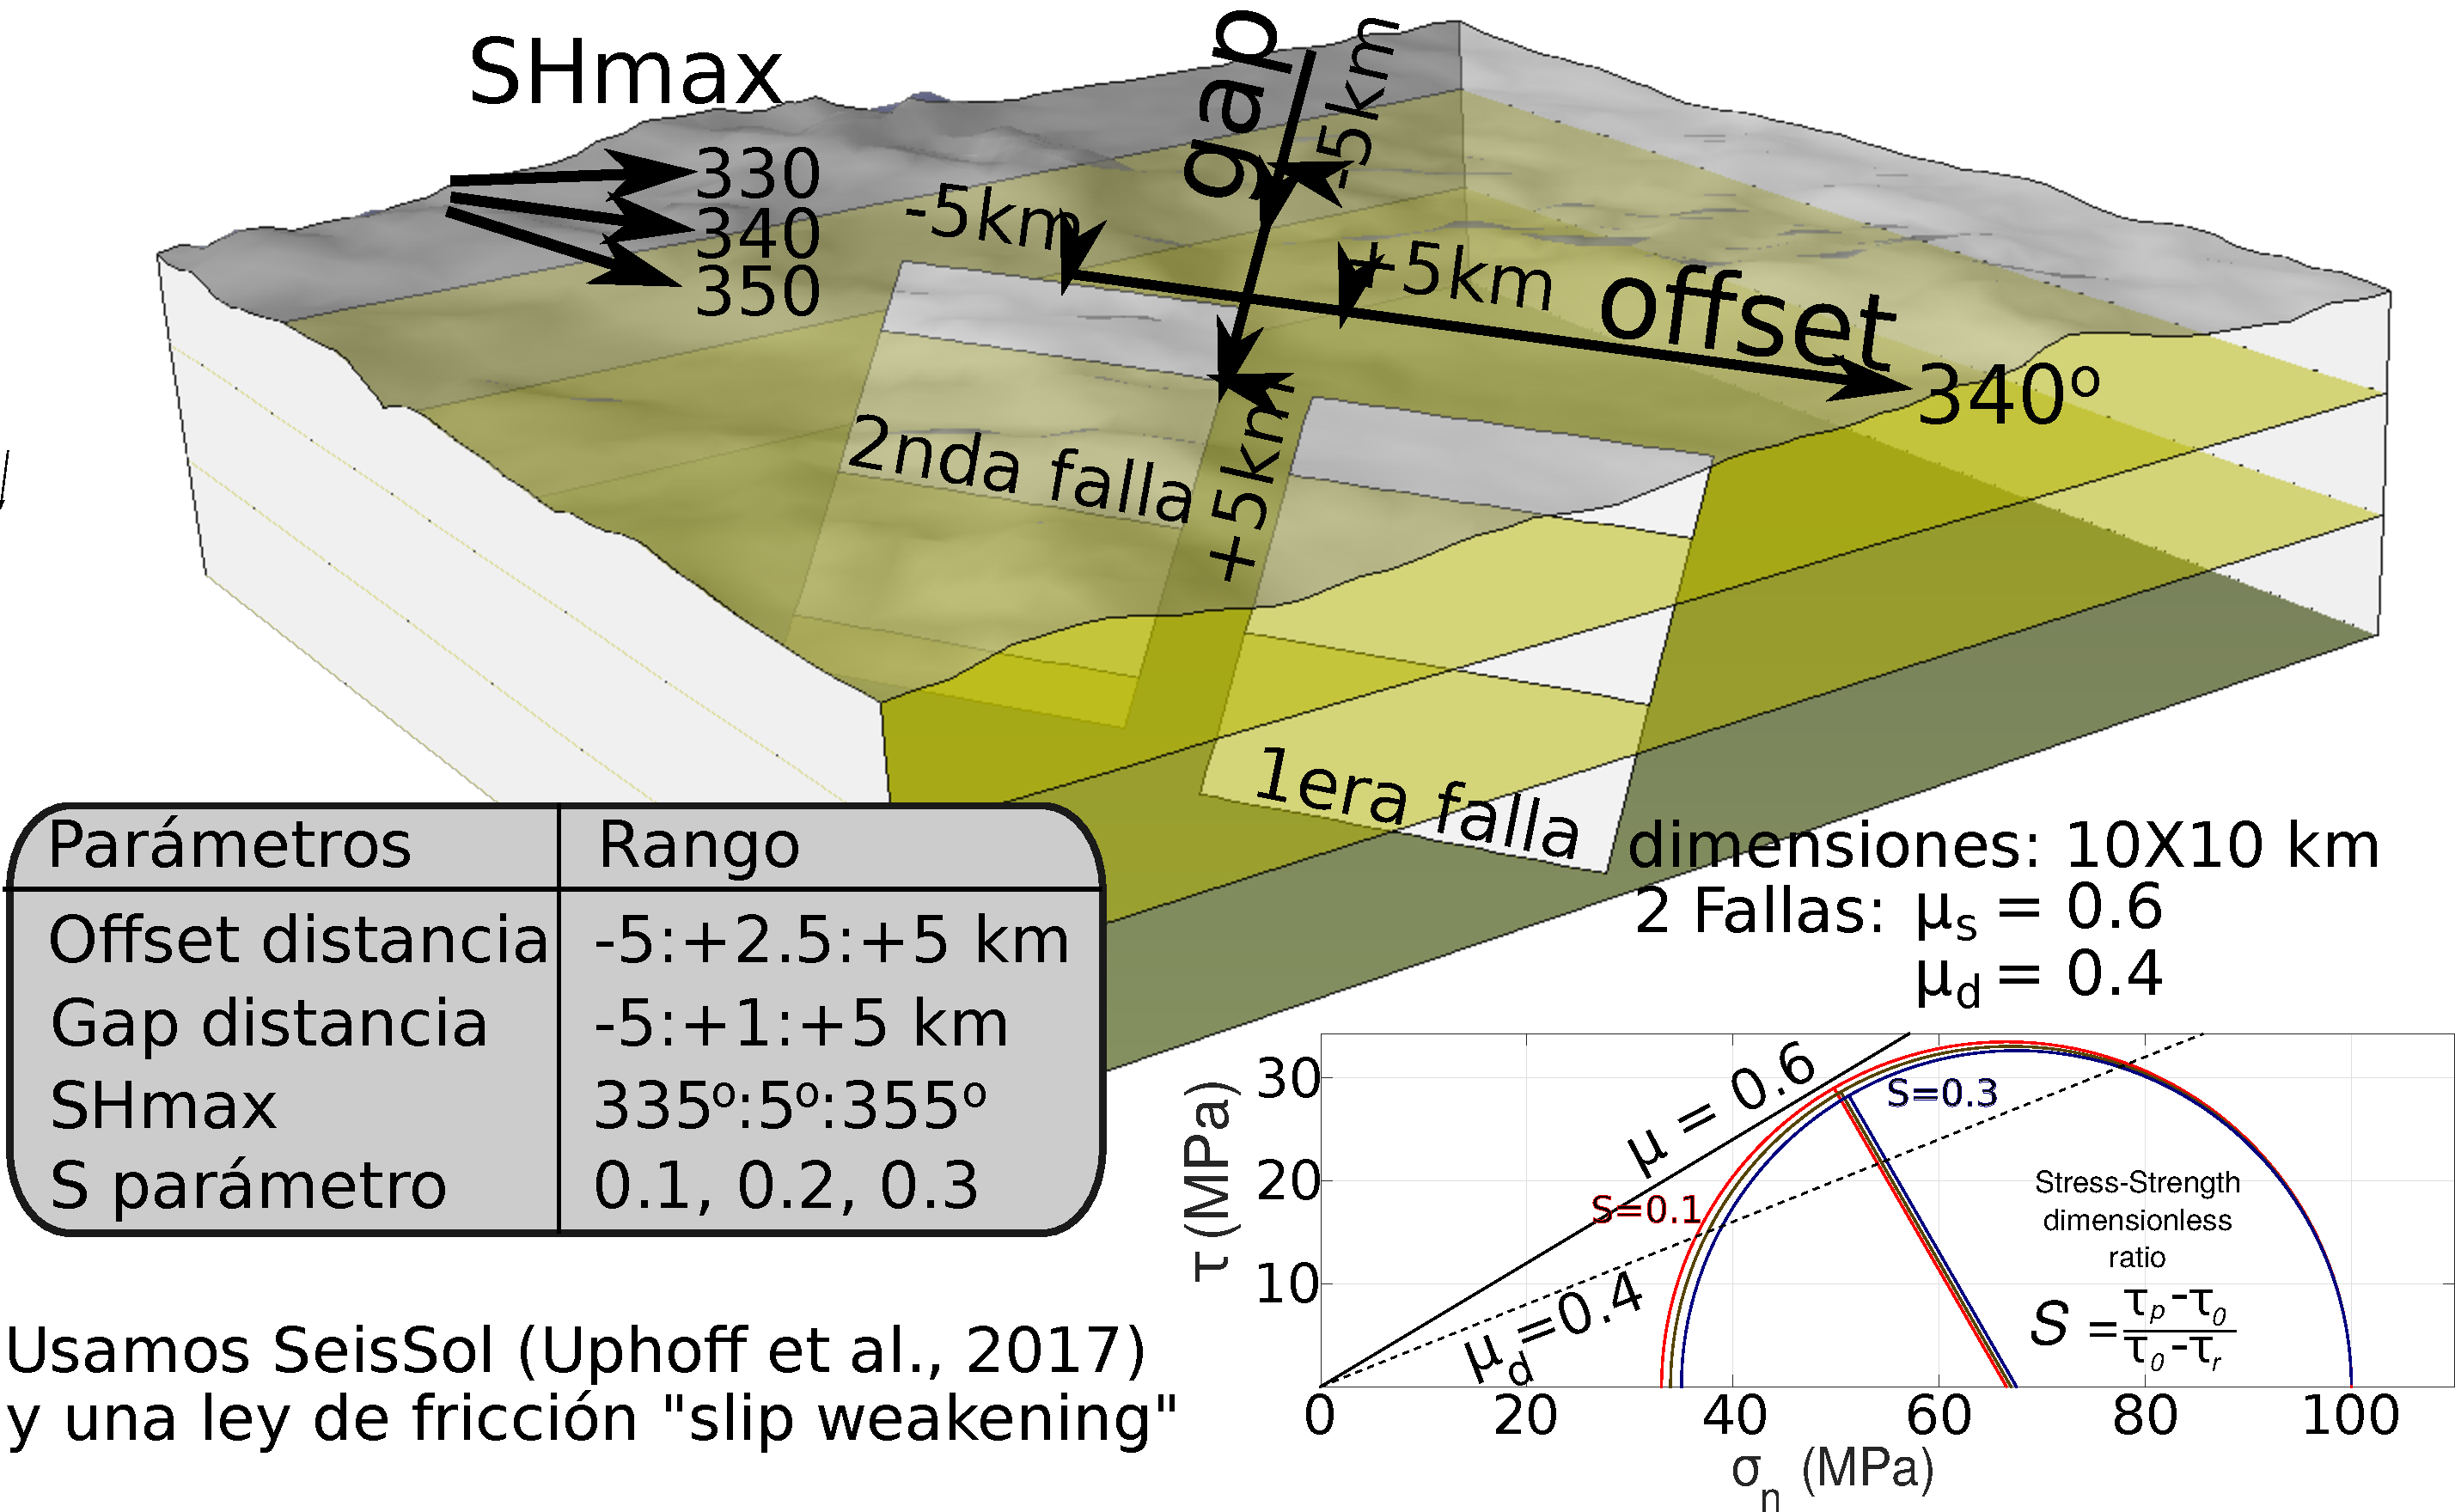
\includegraphics[width=1\linewidth]{images/model.pdf}
\vskip 0.3cm
%\begin{center}
% 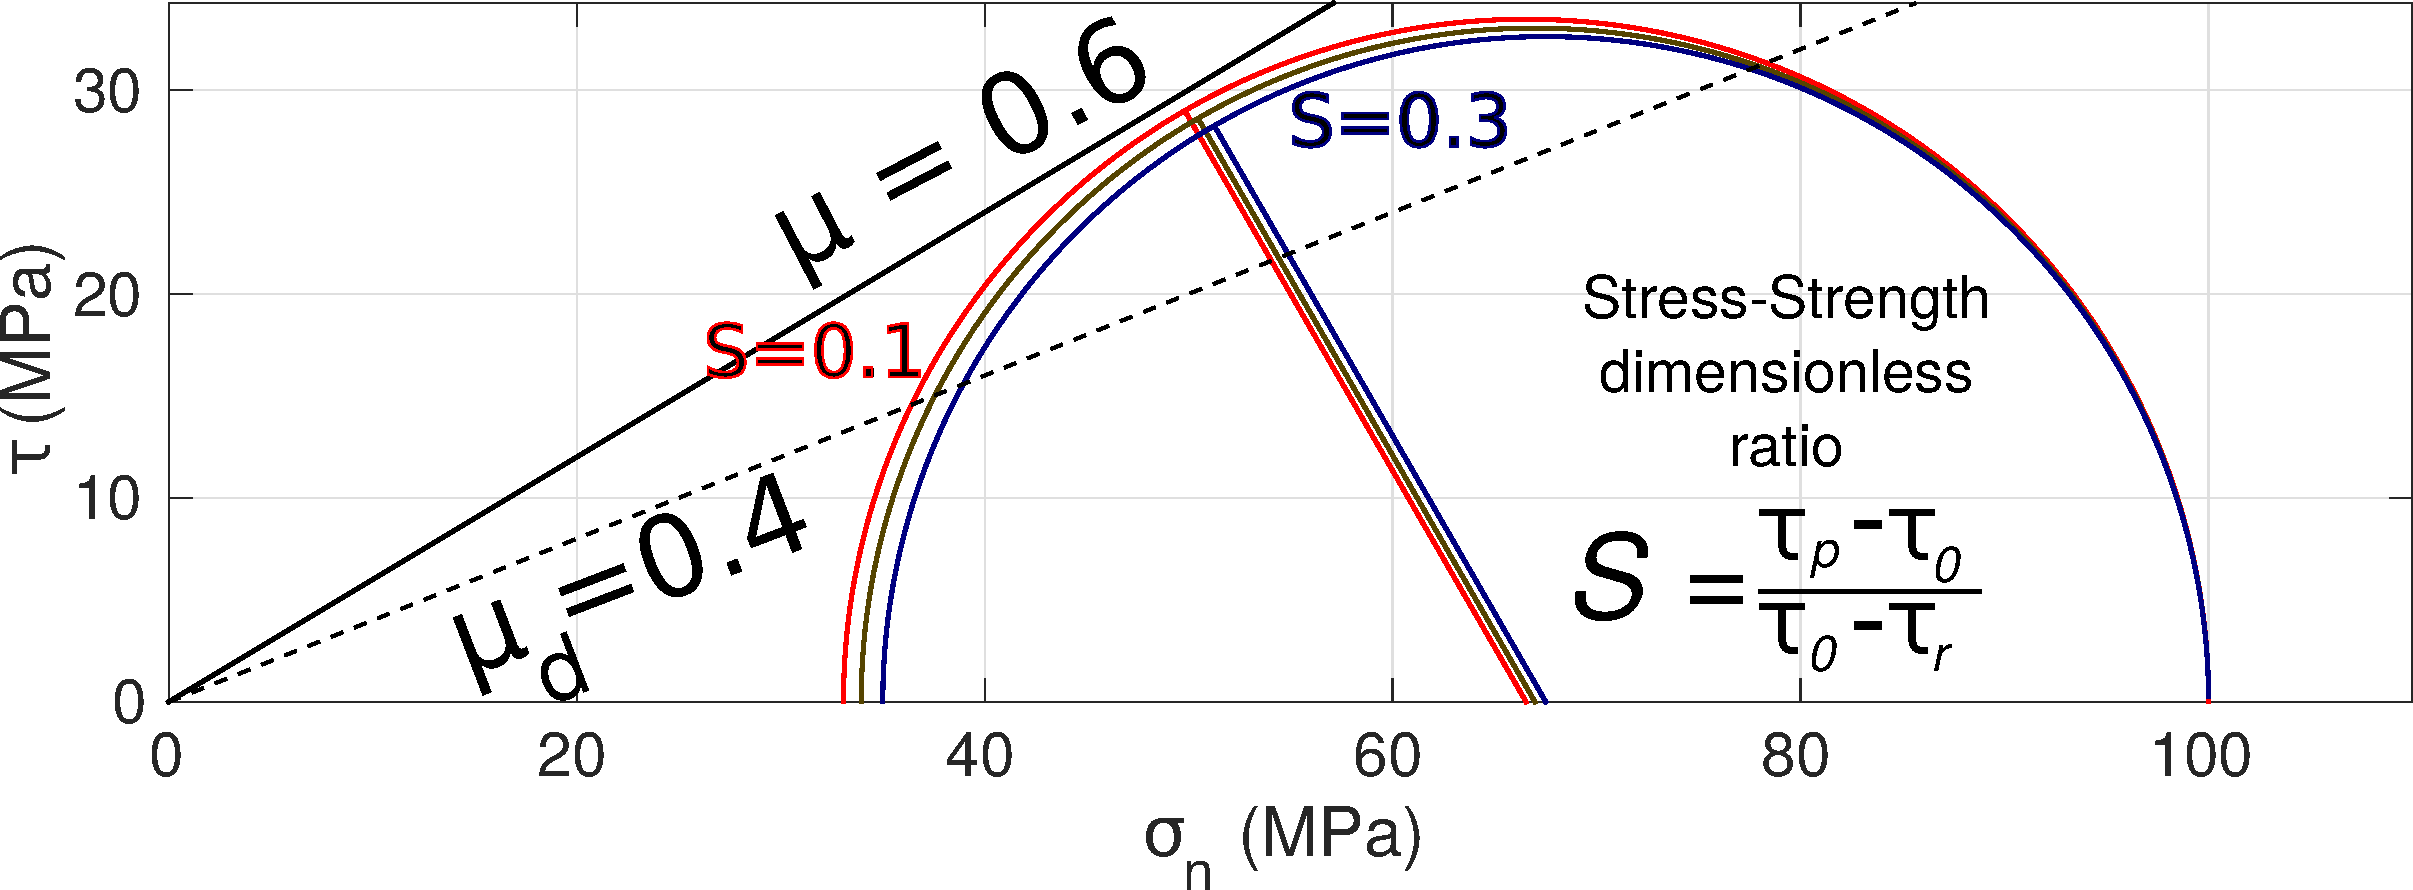
\includegraphics[width=0.75\linewidth]{images/MC_circle_new.pdf} 
%\end{center}
}



\headerbox{{\bf 3.} Resultado de las simulaciones}{name=summary,column=0,row=2,span=1,below=geo}{

\begin{minipage}{1\linewidth}
\vskip -0cm \centering 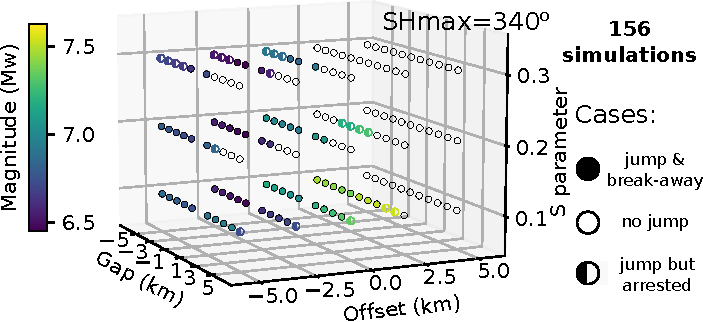
\includegraphics[width=1\linewidth]{images/tests_shmax340.pdf}
\end{minipage} 
\vskip 0.05cm

   \begin{tikzpicture}[% 
    auto,
    block/.style={
      rectangle,
      draw=white!200,
      thick,
      fill=none,
      text width=1\textwidth,
      align=justify,
      rounded corners,
      minimum height=4em,
      minimum width=1\linewidth
    }
  ]
    \draw (2.5,-2) node[block] (C) {
    \small \bf Algunos casos no rompieron la
    segunda falla, debido a la gran distancia entre fallas
    (offset y gap). Este efecto es acentuado en reg\'imenes
    con besfuerzos. El traslapa promueve el salto } ;     
    \draw (2.5,-4.1) node[block] (C) {
    \small \bf Asimetr\'ia (bloques de techo/piso): \\ \vskip -0.3cm
    Cuando la falla secundaria est\'a en el bloque techo
    (con respecto a la primera falla), la ruptura ocasionada
    por la primera falla es m\'as suceptible a generar una 
    ruptura sostenida por m\'as tiempo.} ;
    \draw (2.5,-7.0) node[block] (C) {
    \small \bf Ensombrecimiento de esfuerzos: \\ \vskip -0.3cm
    La energ\'ia total liberada (M$_w$)
    incremeta/disminuye de forma directamente proporcional
    a la distance entre fallas (offset y gap).
    Mientras el traslape incrementa el potencial de 
    salto, el ensombrecimiento de esfuerzos, debido 
    a la proximidad entre fallas, previene una gran
    caida de esfuerzos en la segunda falla.};

  \end{tikzpicture} \vskip -0.2cm

}

\headerbox{{\bf 4.} ¿Salt\'o? ¿C\'omo? ¿C\'uando? ¿Por qu\'e?}{name=snaps,column=1,row=0,span=2}{

\begin{minipage}{1\linewidth}
\vskip -0.0cm \centering {\bf Fault not fixed ($\mu_s=0.6$) \qquad (dynamic analysis)} \vskip 0.1cm
 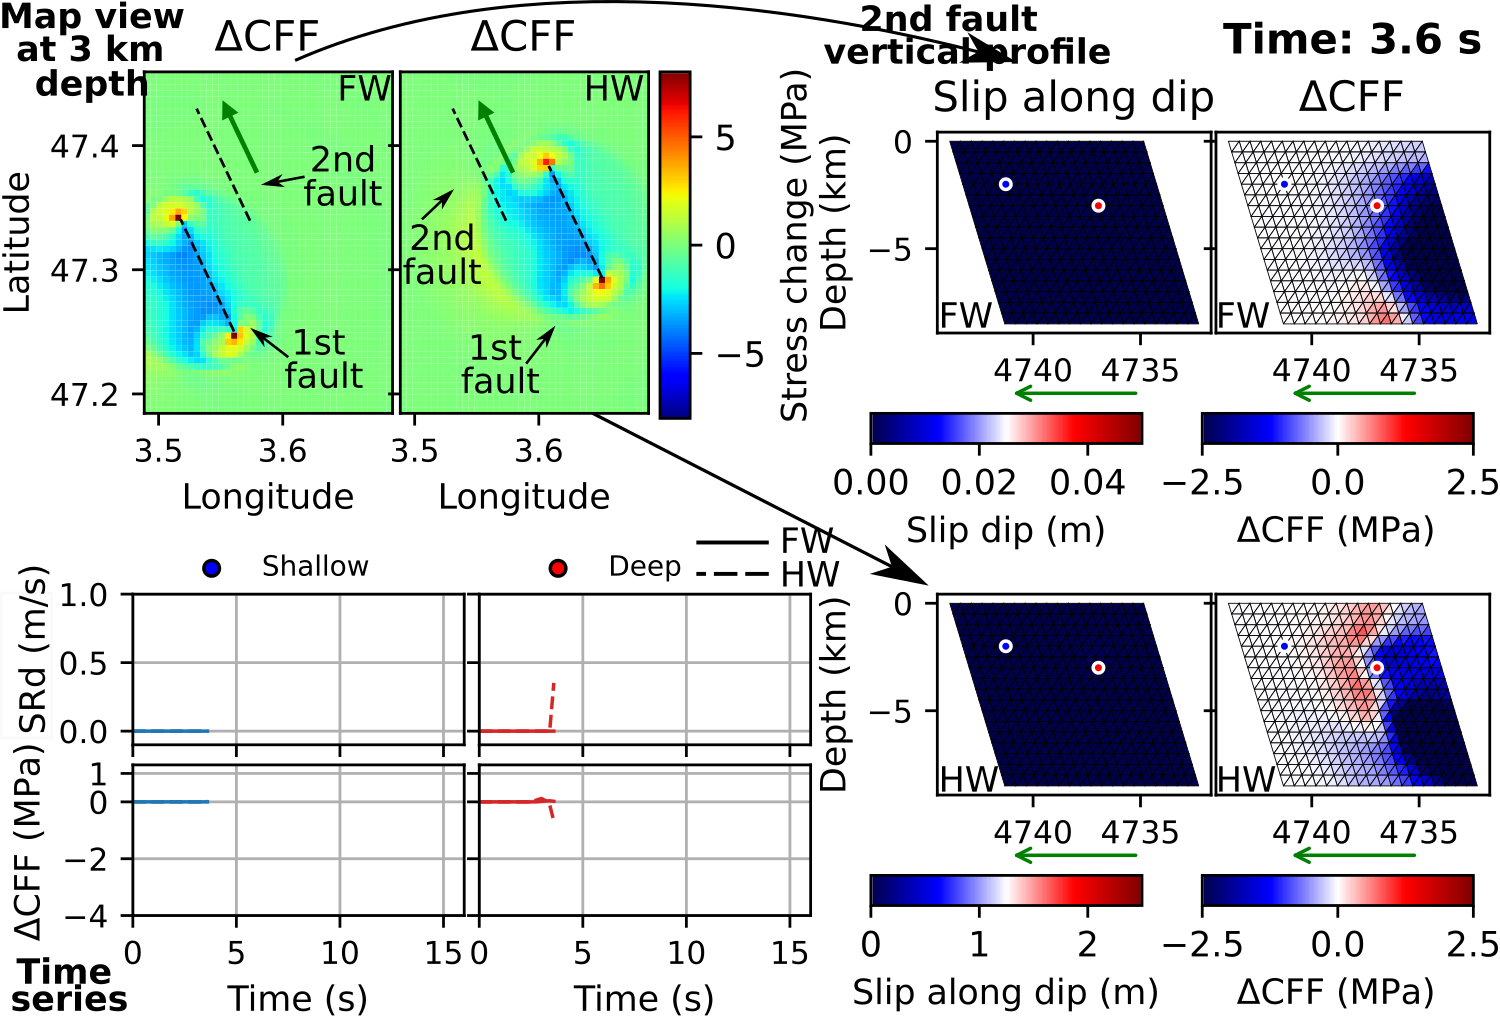
\includegraphics[width=0.8\linewidth]{images/horizontal_delta_00018_nofix.png}
\vskip 0.2cm
\hrule height 0.05cm
\vskip 0.2cm
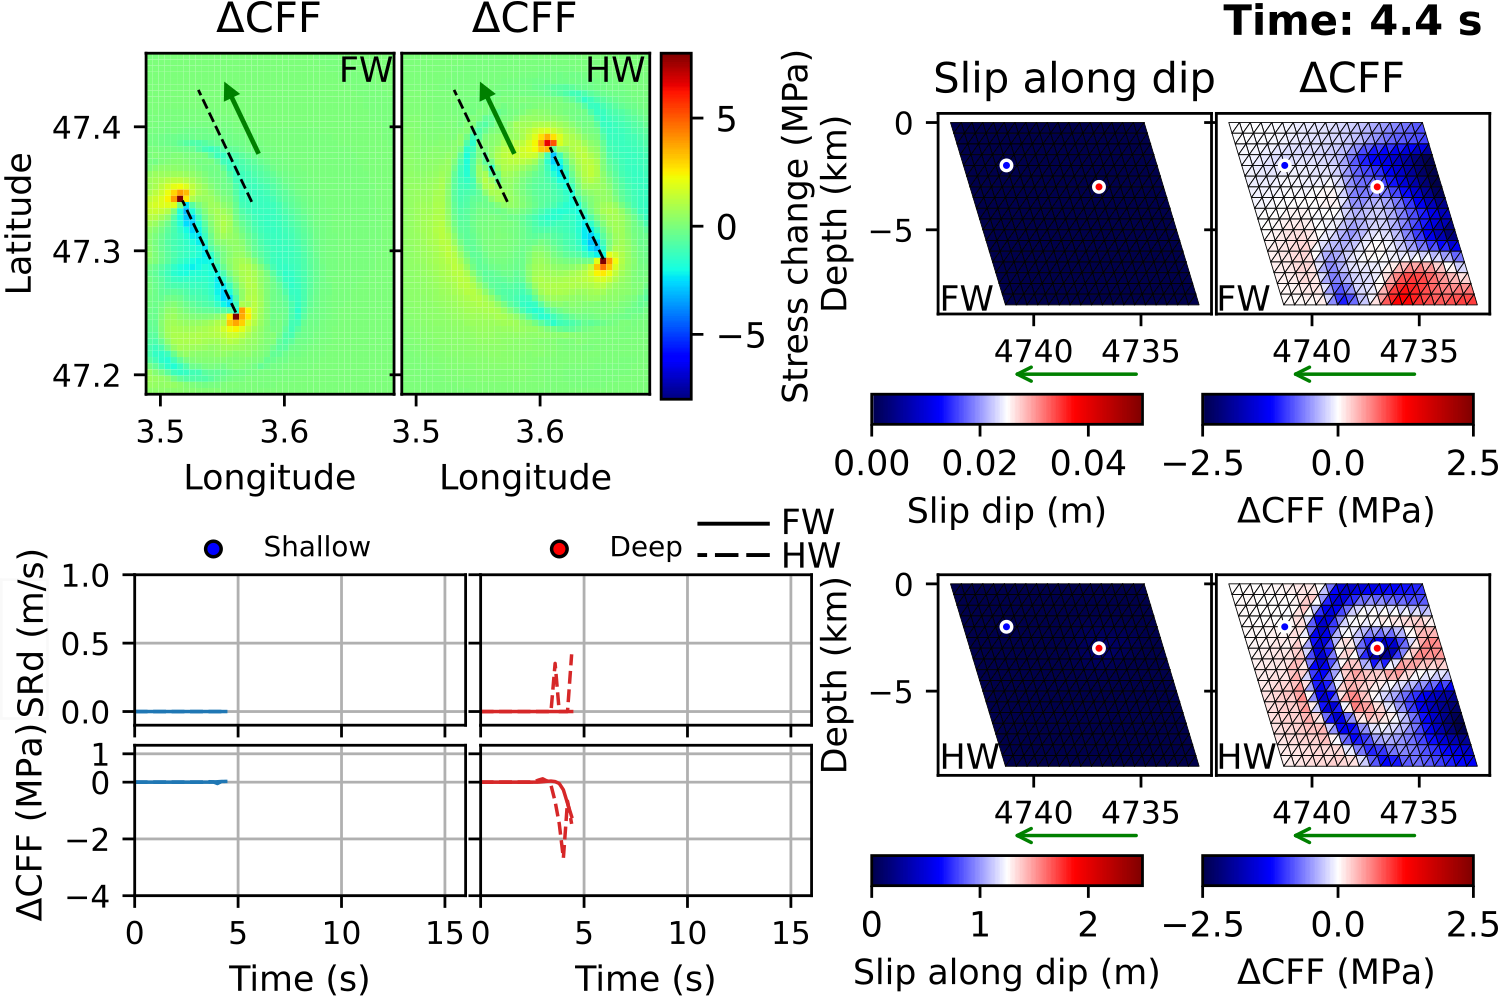
\includegraphics[width=0.8\linewidth]{images/horizontal_delta_00022_nofix.png} \\
\vskip 0.2cm
\hrule height 0.05cm
\vskip 0.2cm
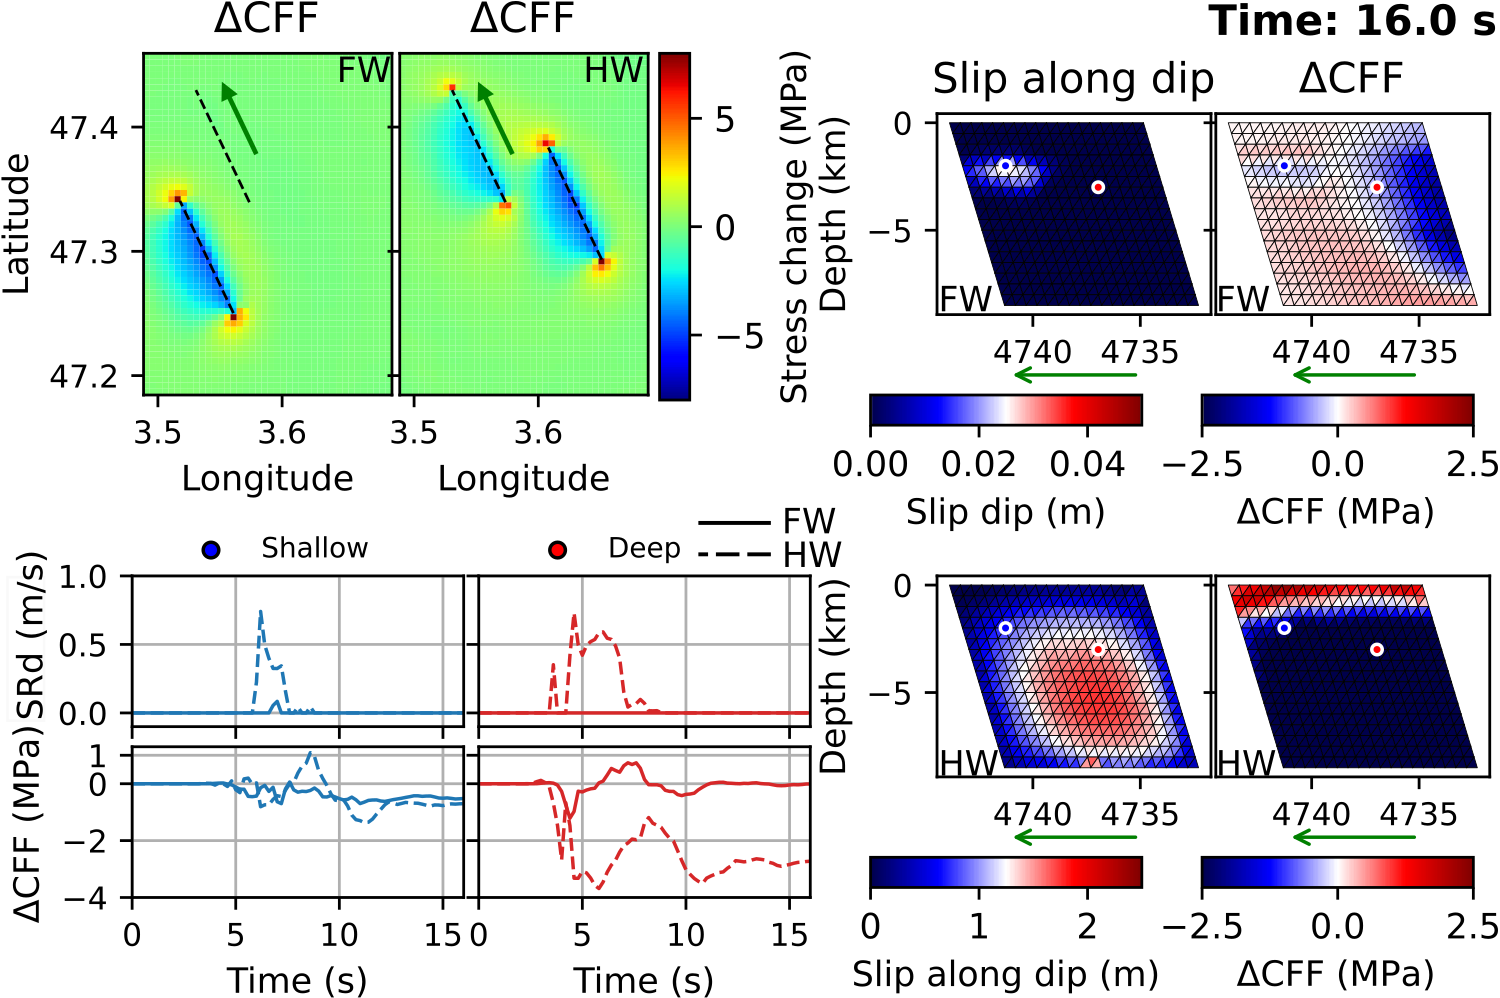
\includegraphics[width=0.8\linewidth]{images/horizontal_delta_00080_nofix.png} 
\end{minipage} \vrule width 0.05cm
%\begin{minipage}{0.32\linewidth}
%\vskip 0.1cm
%\centering Slip rate snapshots \\
%fault not fixed \& \\ break-away behavior \\
%\vskip 0.15cm
%\centering 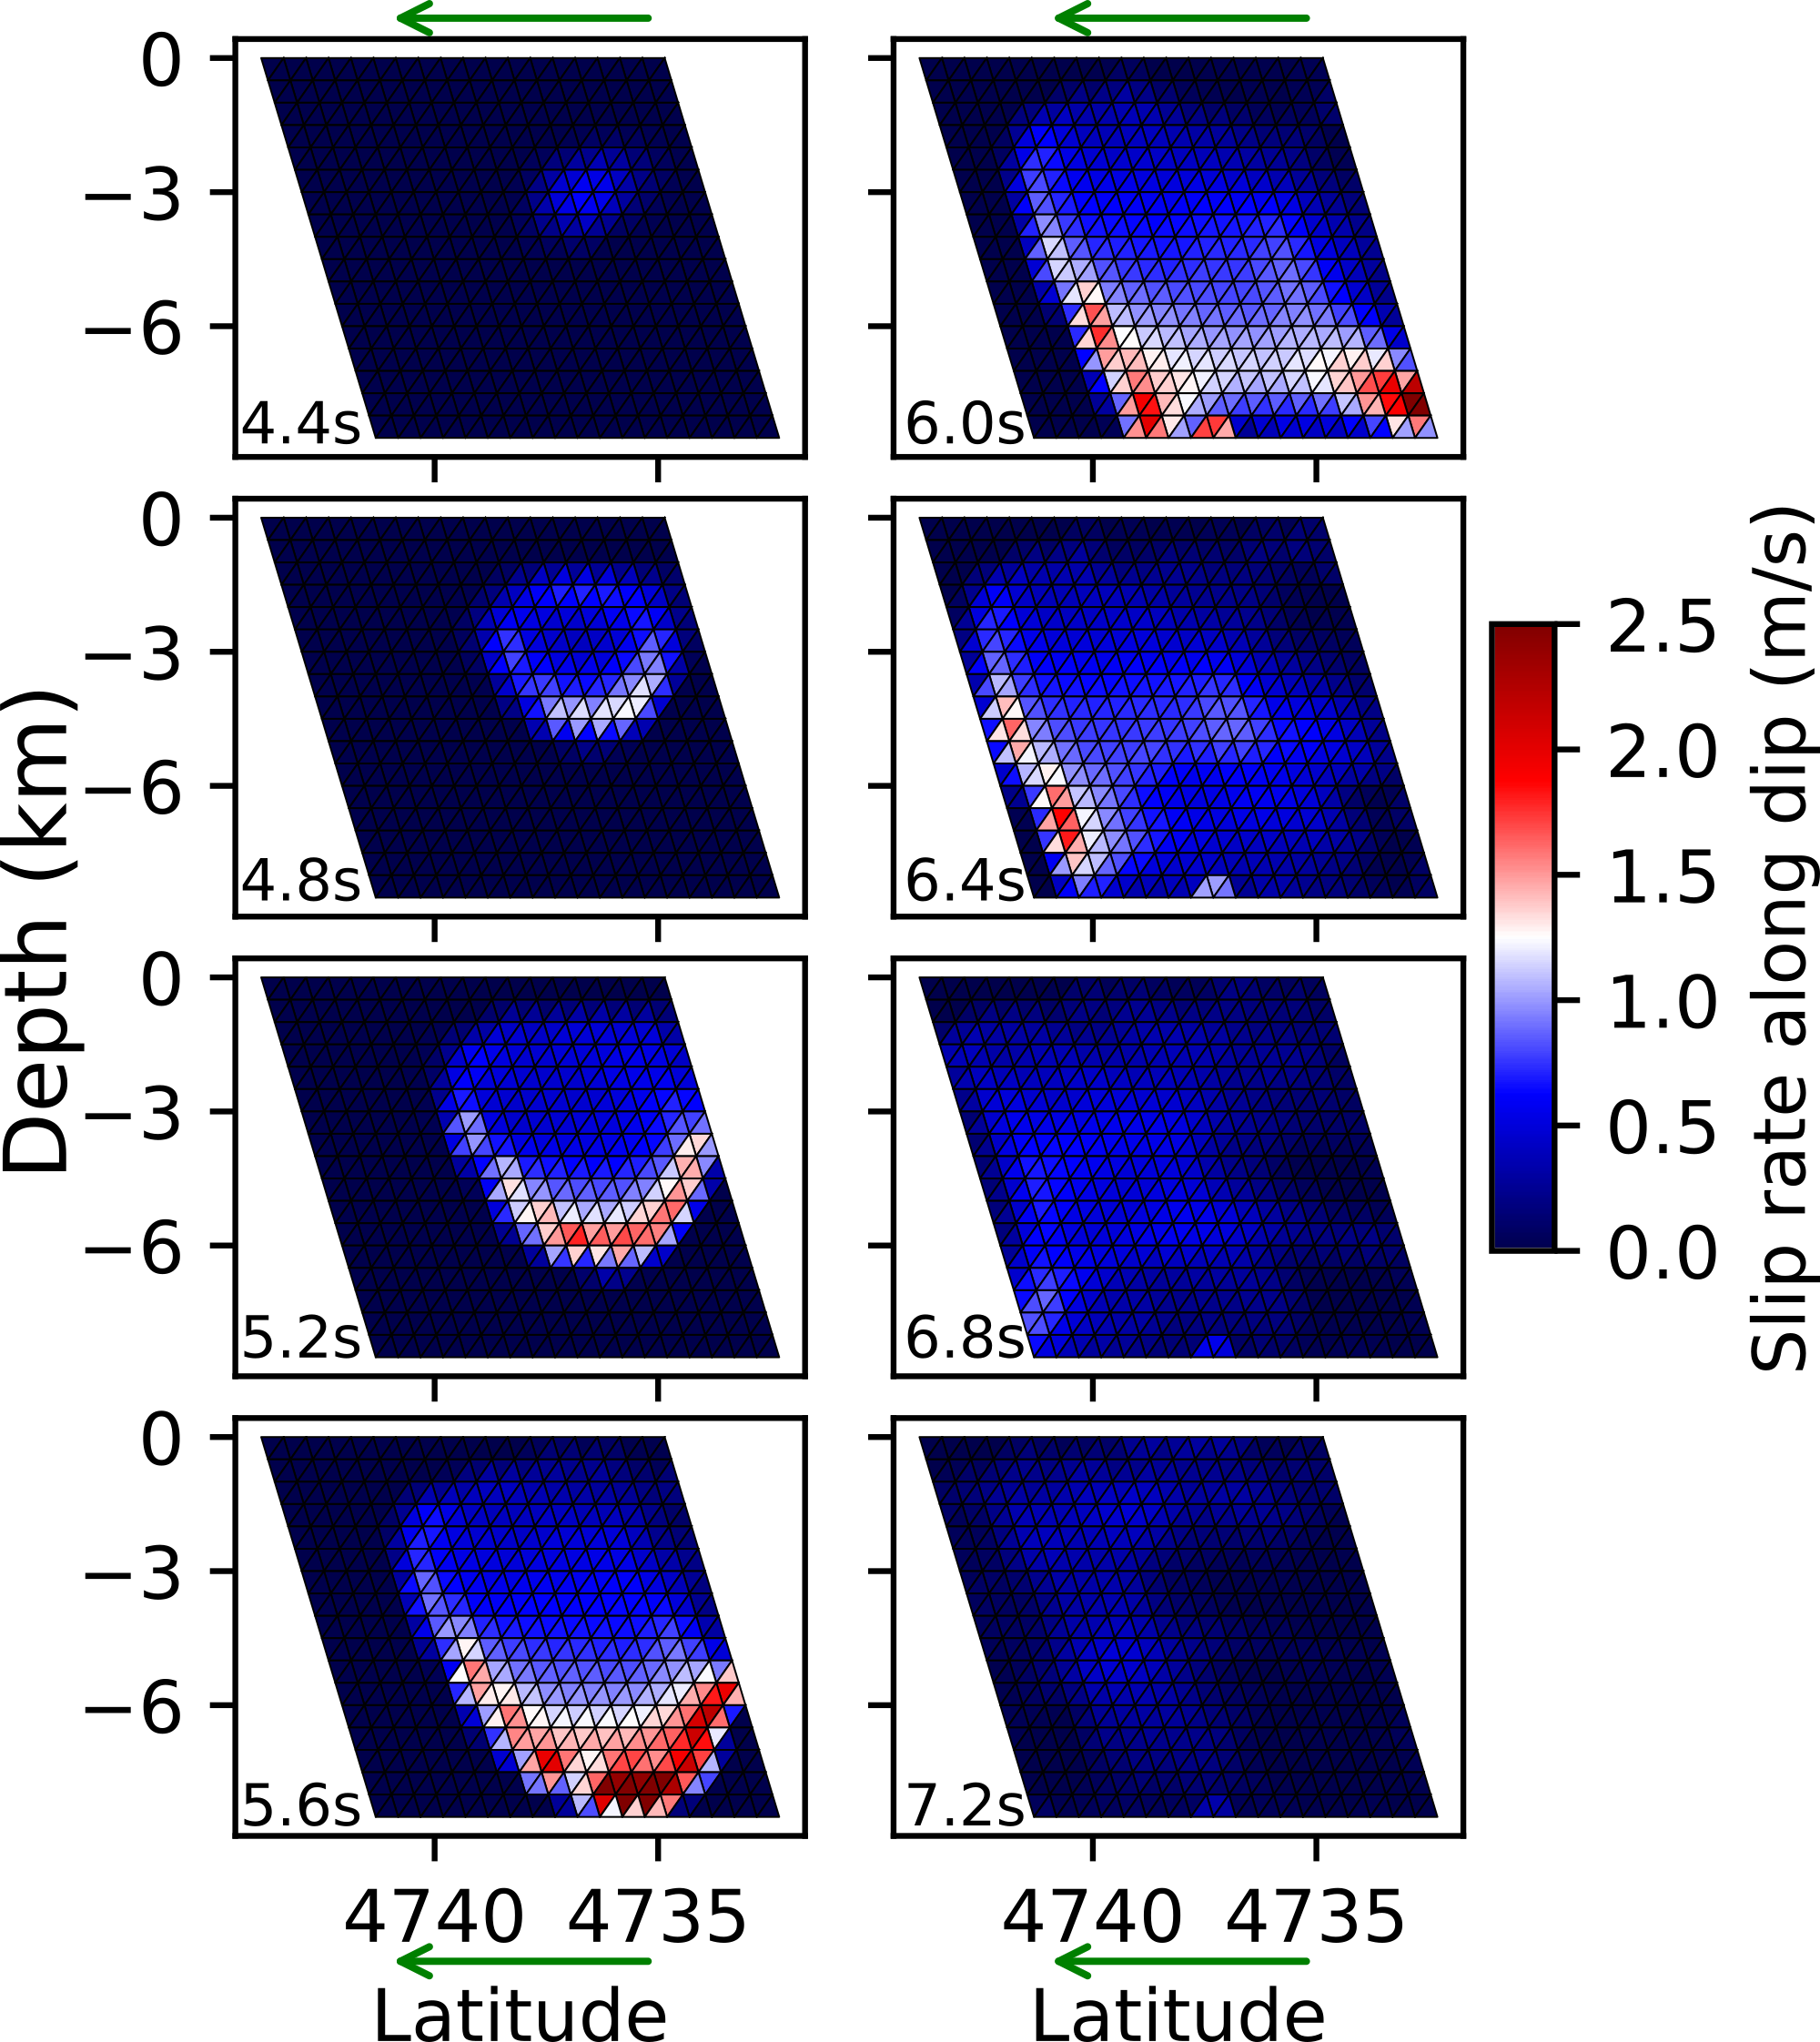
\includegraphics[width=0.95\linewidth]{images/snaps_00080.png}
%\vskip 0.45cm
%\hrule height 0.05cm
%\vskip 0.2cm
% \centering {\bf Fault fixed ($\mu_s=50.0$)} \\
% (static analysis) \vskip 0.2cm
% \includegraphics[width=0.87\linewidth]{images/%horizontal_delta_00080_fix_1.png}
%\vskip 0.2cm
%\vskip 0.2cm
%\includegraphics[width=0.87\linewidth]{images/%horizontal_delta_00080_fix_2.png} \\
%\vskip 0.2cm
%\vskip 0.2cm
%\includegraphics[width=0.87\linewidth]{images/%horizontal_delta_00080_fix_3.png} 
%\end{minipage}
}

\headerbox{{\bf 5.} Conclusi\'on \& Discusion}{name=obs,column=1,row=2,span=1,below=snaps}{
\vskip -0.1cm
\ding{43} El an\'alisis est\'atico es insuficiente para determi-\\
          nar el comportamiento sostenido de la 2nda falla.\\
\vskip -0.4cm
\ding{43} {\bf 5 km} parece la m\'axima distancia que puede sal-\\
          tar la ruptura y continuar de forma sostenida (en \\
          altos niveles de esfuerzo) sin encontrar osbt\'aculos \\
          (direcci\'on SHmax, barreras de fricci\'on, rugosidades).\\
\vskip -0.4cm
\ding{43} {\bf Las rupturas sostenidas} en la 2nda falla pare-\\
           cen ser iniciadas por el arribo simult\'aneo y positiva-\\
           mente onstructivo de dos ondas S provenientes del \\
           fondo y parte norte de la 1era falla. \\
\vskip -0.4cm
\ding{43} Las \'areas positivas de $\Delta$CFF en la 2nda falla no \\ garantizan que la ruptura ser\'a iniciada o sostenida. \\
\vskip -0.4cm
\ding{43} La 2nda falla rompe debido al arribo simult\'aneo\\ de ondas S?
}


\headerbox{\,}{name=ref,column=2,row=2,span=1,above=bottom}{

\nocite{Improta_2019_AVN}
\nocite{Bernard_1989_IRPINIA}
\nocite{Valoroso_2013_AQUILA}
\nocite{Uphoff_2017_ESM}
\vskip -0.7cm
    \setlength{\bibsep}{5pt plus 0.2ex} {\tiny
    \begin{spacing}{1.2}
    \bibliography{biblio/bibtemp} 
    \end{spacing}
    }							
    \bibliographystyle{apalike}    
}

\end{poster}
\end{document}

 









%\headerbox{{\bf 5.} Results}{name=results,column=1,row=2,span=1,above=bottom}{

%}






